%\section{Afsnit}
%\subsection{Thomas}
%% the license
%\begin{frame}{Afsnit}{Thomas}
%  \begin{itemize}
%    \item<1-> TEST
%  \end{itemize}
%\end{frame}
%%%%%%%%%%%%%%%%%

\section{Regulatorer}
%%%%%%%%%%%% MID WAY AGENDA %%%%%%%%%%%%%%
\begin{frame}<beamer>
\frametitle{Thomas Holm Pilgaard}
\tableofcontents[currentsection]
\end{frame}
%%%%%%%%%%%% MID WAY AGENDA %%%%%%%%%%%%%%


% \begin{frame}{Regulator}{Klassisk regulator design}


% \begin{columns}[T]
% \begin{column}{.35\textwidth}
% \vspace{2cm}
%   \begin{itemize}
%     \item<1-> S domænet
%         \begin{itemize}
%           \item<1-> 
%           \item<1-> bla bla bla
%         \end{itemize}
%   \end{itemize}
% \end{column}%
% \hfill%
% \begin{column}{.65\textwidth}

% \end{column}
% \end{columns}

%   \end{frame}







\begin{frame}{Regulatorer}{Blok diagram}


   % \centering
   % \begin{minipage}[t]{0.75\linewidth}
   %   \begin{itemize}
   %     \item<1->[] {
   %             \begin{figure}[H]
   %             \centering
   %             \scalebox{0.65}{\input{Billeder/Thomas/regulatorblock4.ralf}}
   %             \end{figure}
   %     }
   %   \end{itemize}           
   % \end{minipage}
   % \\
  
   % \centering   
   % \begin{minipage}[t]{0.55\linewidth}
    
   %   \begin{itemize}
   %     \item<1->[] {
   %             \begin{figure}[H]
   %             \centering
   %             \scalebox{0.65}{\input{Billeder/Thomas/regulatorblocky.ralf}}
   %             \end{figure}
   %     }
   %   \end{itemize}           
   % \end{minipage}

 \begin{figure}[H]
   \centering
   \scalebox{0.65}{\input{Billeder/Thomas/regulatorblock3.ralf}}
 \end{figure}

 \vspace{5.3}

 \begin{figure}[H]
   \centering
   \scalebox{0.65}{\input{Billeder/Thomas/regulatorblocky.ralf}}
 \end{figure}


% \begin{figure}[H]
%   \centering
%   \onslide<1-> \scalebox{0.65}{\input{Billeder/Thomas/regulatorblock3.ralf}}
% \end{figure}

% \vspace{5.3}

% \begin{figure}[H]
%   \centering
%   \onslide<2-> \scalebox{0.65}{\input{Billeder/Thomas/regulatorblocky.ralf}}
% \end{figure}



\end{frame}

\begin{frame}{Regulatorer}{Root locus vinkel}
\vspace{1cm}
\begin{figure}[H]
\centering
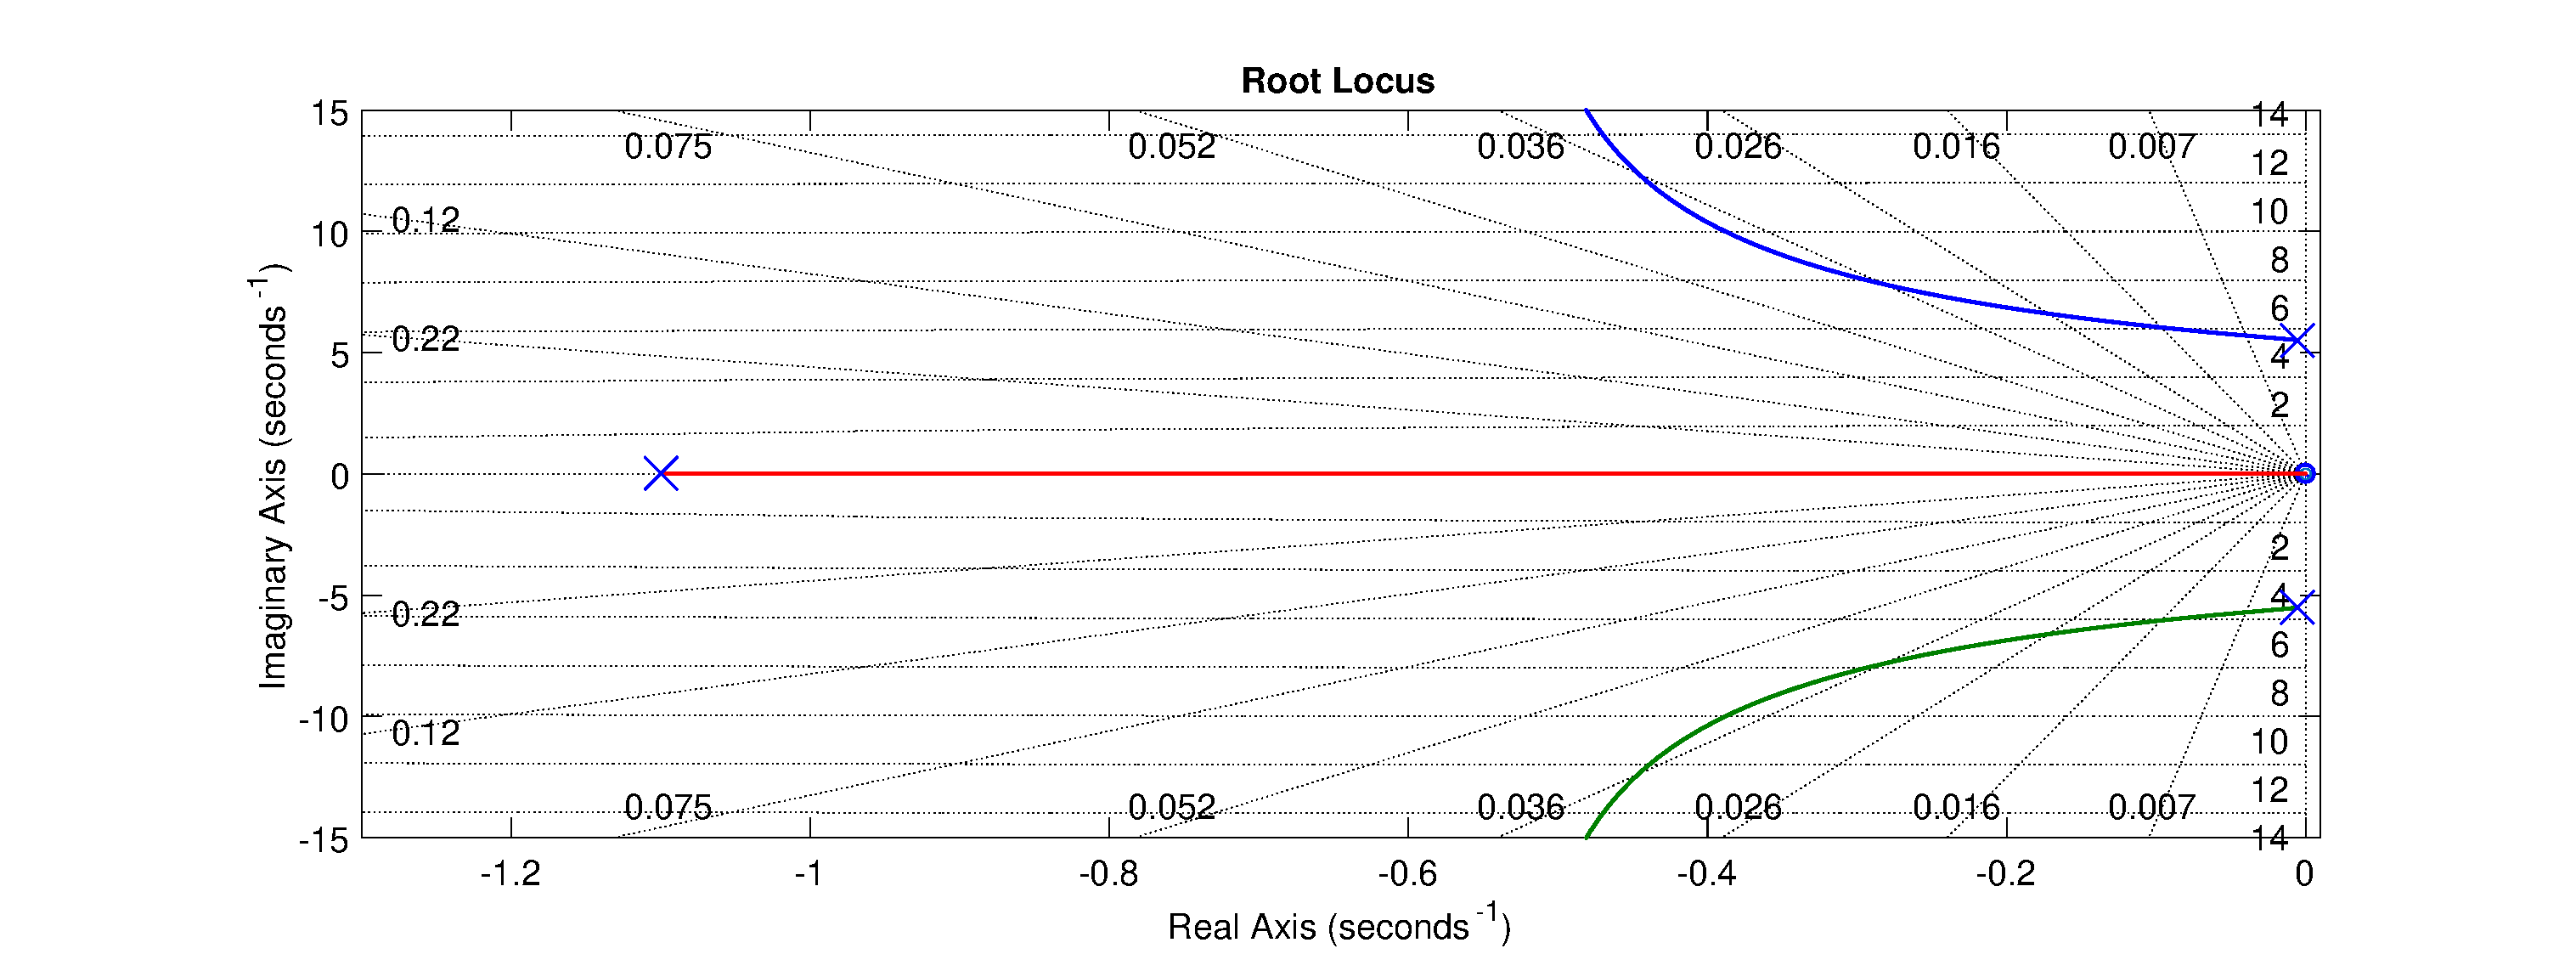
\includegraphics[width=1\textwidth]{billeder/Thomas/AngleConRL11}
\end{figure}
\end{frame}


\begin{frame}{Regulatorer}{Root locus vinkel}
\vspace{1cm}
\begin{figure}[H]
\centering
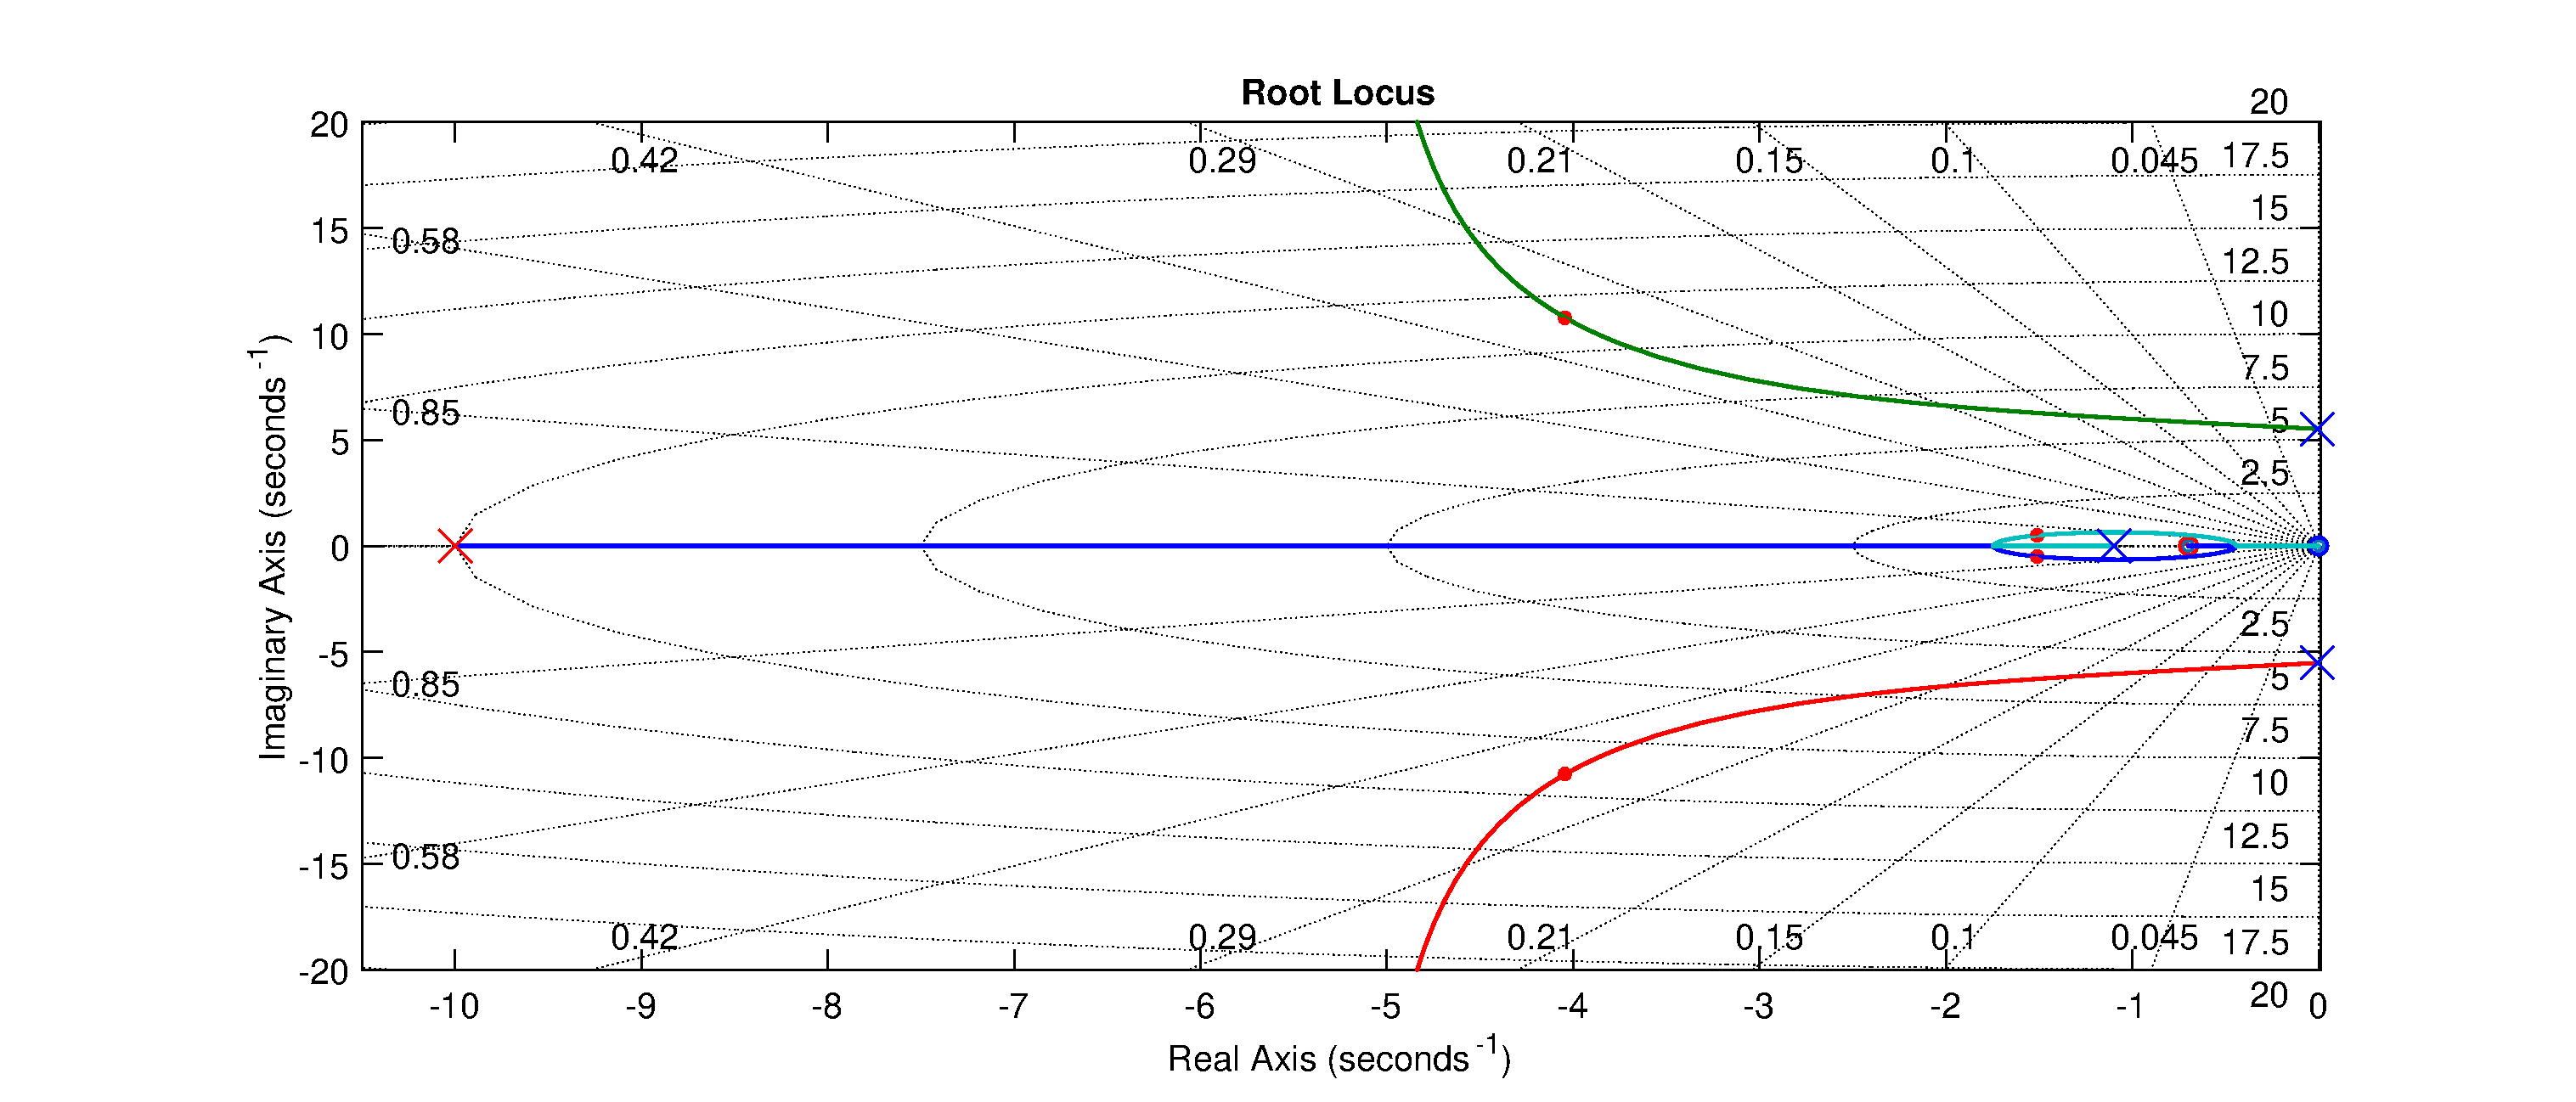
\includegraphics[width=1\textwidth]{Billeder/Thomas/AngleOpenLoop}
\end{figure}
\end{frame}

\begin{frame}{Regulatorer}{Closed loop step respons vinkel}
\begin{figure}[H]
\vspace{1.5cm}
\centering
%\includegraphics[width=0.9\textwidth]{Billeder/Thomas/AngleClosedloopstep}
%\scalebox{0.8} {
% This file was created by matlab2tikz.
%
%The latest updates can be retrieved from
%  http://www.mathworks.com/matlabcentral/fileexchange/22022-matlab2tikz-matlab2tikz
%where you can also make suggestions and rate matlab2tikz.
%
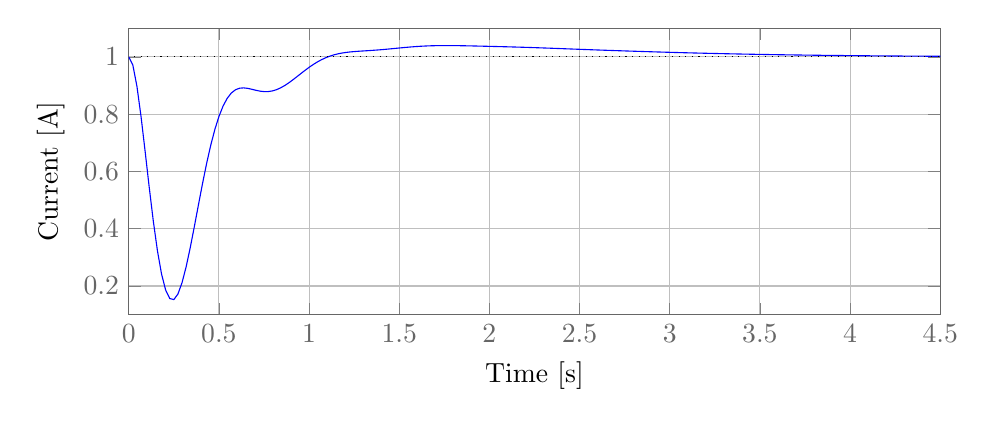
\begin{tikzpicture}

\begin{axis}[%
width=0.85\textwidth,
height=0.3\textwidth,
at={(1.975in,0.746in)},
scale only axis,
separate axis lines,
every outer x axis line/.append style={white!40!black},
every x tick label/.append style={font=\color{white!40!black}},
xmin=0,
xmax=4.5,
xmajorgrids,
xlabel={Time [s]},
every outer y axis line/.append style={white!40!black},
every y tick label/.append style={font=\color{white!40!black}},
ymin=0.1,
ymax=1.1,
ymajorgrids,
ylabel={Current [A]},
axis background/.style={fill=white}
]
\addplot [color=blue,solid,forget plot]
  table[row sep=crcr]{%
0	1\\
0.0227528486535158	0.971859342603638\\
0.0455056973070316	0.897524231115418\\
0.0682585459605474	0.792150043886678\\
0.0910113946140632	0.670163067738347\\
0.113764243267579	0.544486412878134\\
0.136517091921095	0.425989911749438\\
0.159269940574611	0.323160692862605\\
0.182022789228126	0.241977890238838\\
0.204775637881642	0.185964977835278\\
0.227528486535158	0.156386580876281\\
0.250281335188674	0.152553166204965\\
0.27303418384219	0.172196430847109\\
0.295787032495705	0.211880046050608\\
0.318539881149221	0.267414150993223\\
0.341292729802737	0.334247073212653\\
0.364045578456253	0.407813637612809\\
0.386798427109769	0.483825610062481\\
0.409551275763284	0.558495868399752\\
0.4323041244168	0.628693448415354\\
0.455056973070316	0.69203141084787\\
0.477809821723832	0.746893345030093\\
0.500562670377348	0.792407180086614\\
0.523315519030863	0.828376807761253\\
0.546068367684379	0.855182889470085\\
0.568821216337895	0.873664232060762\\
0.591574064991411	0.884990415385541\\
0.614326913644927	0.89053510397904\\
0.637079762298443	0.891757845454882\\
0.659832610951958	0.890100315252366\\
0.682585459605474	0.886901062103816\\
0.70533830825899	0.883330970566316\\
0.728091156912506	0.880349989690254\\
0.750844005566021	0.87868425581915\\
0.773596854219537	0.878821609995853\\
0.796349702873053	0.881022697545281\\
0.819102551526569	0.885344336971374\\
0.841855400180085	0.891671636041704\\
0.864608248833601	0.899755378926245\\
0.887361097487116	0.909251463690159\\
0.910113946140632	0.91975958311996\\
0.932866794794148	0.930858861320235\\
0.955619643447664	0.942138733504533\\
0.978372492101179	0.953223941654054\\
1.0011253407547	0.963793075940382\\
1.02387818940821	0.973590590905626\\
1.04663103806173	0.982432644961956\\
1.06938388671524	0.990207438979097\\
1.09213673536876	0.996870959668754\\
1.11488958402227	1.00243916814705\\
1.13764243267579	1.00697772107355\\
1.16039528132931	1.01059028293757\\
1.18314812998282	1.01340639794986\\
1.20590097863634	1.01556975454151\\
1.22865382728985	1.01722751076157\\
1.25140667594337	1.01852117011482\\
1.27415952459689	1.01957931811851\\
1.2969123732504	1.02051236136967\\
1.31966522190392	1.02140926191499\\
1.34241807055743	1.02233613623442\\
1.36517091921095	1.02333649360878\\
1.38792376786446	1.02443282407827\\
1.41067661651798	1.02562921060417\\
1.4334294651715	1.0269146307687\\
1.45618231382501	1.02826662654221\\
1.47893516247853	1.02965505170559\\
1.50168801113204	1.03104565049479\\
1.52444085978556	1.03240327301125\\
1.54719370843907	1.03369458832426\\
1.56994655709259	1.03489021094625\\
1.59269940574611	1.03596620717336\\
1.61545225439962	1.03690499214155\\
1.63820510305314	1.03769566466607\\
1.66095795170665	1.03833385411714\\
1.68371080036017	1.03882117155764\\
1.70646364901369	1.03916436655656\\
1.7292164976672	1.03937429239917\\
1.75196934632072	1.03946477708488\\
1.77472219497423	1.03945148698639\\
1.79747504362775	1.03935085586951\\
1.82022789228126	1.03917913564089\\
1.84298074093478	1.03895160808656\\
1.8657335895883	1.0386819801841\\
1.88848643824181	1.03838197028746\\
1.91123928689533	1.03806107931539\\
1.93399213554884	1.03772653048864\\
1.95674498420236	1.03738335338537\\
1.97949783285587	1.03703458313001\\
2.00225068150939	1.03668154323504\\
2.02500353016291	1.03632418067177\\
2.04775637881642	1.03596142375786\\
2.07050922746994	1.03559153695995\\
2.09326207612345	1.03521245124878\\
2.11601492477697	1.03482205375438\\
2.13876777343049	1.03441842573545\\
2.161520622084	1.0340000229439\\
2.18427347073752	1.0335657970507\\
2.20702631939103	1.03311526069578\\
2.22977916804455	1.03264850180705\\
2.25253201669806	1.03216615504416\\
2.27528486535158	1.03166933957118\\
2.2980377140051	1.03115957290934\\
2.32079056265861	1.0306386704669\\
2.34354341131213	1.03010863961583\\
2.36629625996564	1.02957157602595\\
2.38904910861916	1.02902956852197\\
2.41180195727268	1.02848461713526\\
2.43455480592619	1.0279385674054\\
2.45730765457971	1.02739306245079\\
2.48006050323322	1.02684951295589\\
2.50281335188674	1.02630908407241\\
2.52556620054025	1.02577269733815\\
2.54831904919377	1.02524104509233\\
2.57107189784729	1.02471461450461\\
2.5938247465008	1.02419371821404\\
2.61657759515432	1.02367852866179\\
2.63933044380783	1.02316911345674\\
2.66208329246135	1.02266546949134\\
2.68483614111486	1.02216755398311\\
2.70758898976838	1.02167531111203\\
2.7303418384219	1.02118869341868\\
2.75309468707541	1.02070767759222\\
2.77584753572893	1.02023227468631\\
2.79860038438244	1.01976253513927\\
2.82135323303596	1.01929854923261\\
2.84410608168948	1.01884044379715\\
2.86685893034299	1.01838837607103\\
2.88961177899651	1.01794252563656\\
2.91236462765002	1.0175030853243\\
2.93511747630354	1.01707025188468\\
2.95787032495705	1.01664421710488\\
2.98062317361057	1.01622515990421\\
3.00337602226409	1.01581323978794\\
3.0261288709176	1.01540859188816\\
3.04888171957112	1.01501132368073\\
3.07163456822463	1.0146215133451\\
3.09438741687815	1.01423920963487\\
3.11714026553167	1.01386443305275\\
3.13989311418518	1.01349717807473\\
3.1626459628387	1.01313741614406\\
3.18539881149221	1.01278509915249\\
3.20815166014573	1.01244016314181\\
3.23090450879924	1.0121025319882\\
3.25365735745276	1.01177212087137\\
3.27641020610628	1.01144883937562\\
3.29916305475979	1.01113259411754\\
3.32191590341331	1.01082329084062\\
3.34466875206682	1.01052083595934\\
3.36742160072034	1.01022513757133\\
3.39017444937385	1.009936105985\\
3.41292729802737	1.00965365383137\\
3.43568014668089	1.00937769584194\\
3.4584329953344	1.00910814838076\\
3.48118584398792	1.00884492881804\\
3.50393869264143	1.00858795482727\\
3.52669154129495	1.00833714367757\\
3.54944438994847	1.00809241158063\\
3.57219723860198	1.00785367313708\\
3.5949500872555	1.00762084091293\\
3.61770293590901	1.00739382516234\\
3.64045578456253	1.00717253370066\\
3.66320863321604	1.00695687192069\\
3.68596148186956	1.00674674293705\\
3.70871433052308	1.00654204783695\\
3.73146717917659	1.00634268601265\\
3.75422002783011	1.0061485555489\\
3.77697287648362	1.00595955363945\\
3.79972572513714	1.00577557700864\\
3.82247857379065	1.00559652231739\\
3.84523142244417	1.00542228653682\\
3.86798427109769	1.00525276727714\\
3.8907371197512	1.00508786306405\\
3.91348996840472	1.00492747355879\\
3.93624281705823	1.00477149972218\\
3.95899566571175	1.00461984392563\\
3.98174851436527	1.00447241001495\\
4.00450136301878	1.00432910333417\\
4.0272542116723	1.00418983071779\\
4.05000706032581	1.00405450045995\\
4.07275990897933	1.0039230222688\\
4.09551275763284	1.00379530721384\\
4.11826560628636	1.00367126767248\\
4.14101845493988	1.00355081728127\\
4.16377130359339	1.00343387089546\\
4.18652415224691	1.00332034455956\\
4.20927700090042	1.00321015548987\\
4.23202984955394	1.00310322206919\\
4.25478269820746	1.00299946385273\\
4.27753554686097	1.00289880158367\\
4.30028839551449	1.00280115721628\\
4.323041244168	1.00270645394423\\
4.34579409282152	1.00261461623172\\
4.36854694147503	1.00252556984512\\
4.39129979012855	1.00243924188299\\
4.41405263878207	1.00235556080296\\
4.43680548743558	1.00227445644383\\
4.4595583360891	1.00219586004231\\
4.48231118474261	1.00211970424361\\
4.50506403339613	1.00204592310599\\
};
\addplot [color=black,dotted,forget plot]
  table[row sep=crcr]{%
-0.45	1\\
0	1\\
1	1\\
4.95000000000005	1\\
};
\end{axis}
\end{tikzpicture}%
%}
\end{figure}
\end{frame}

\begin{frame}{Regulatorer}{Root locus trolley}
\vspace{1cm}
\begin{figure}[H]
\centering
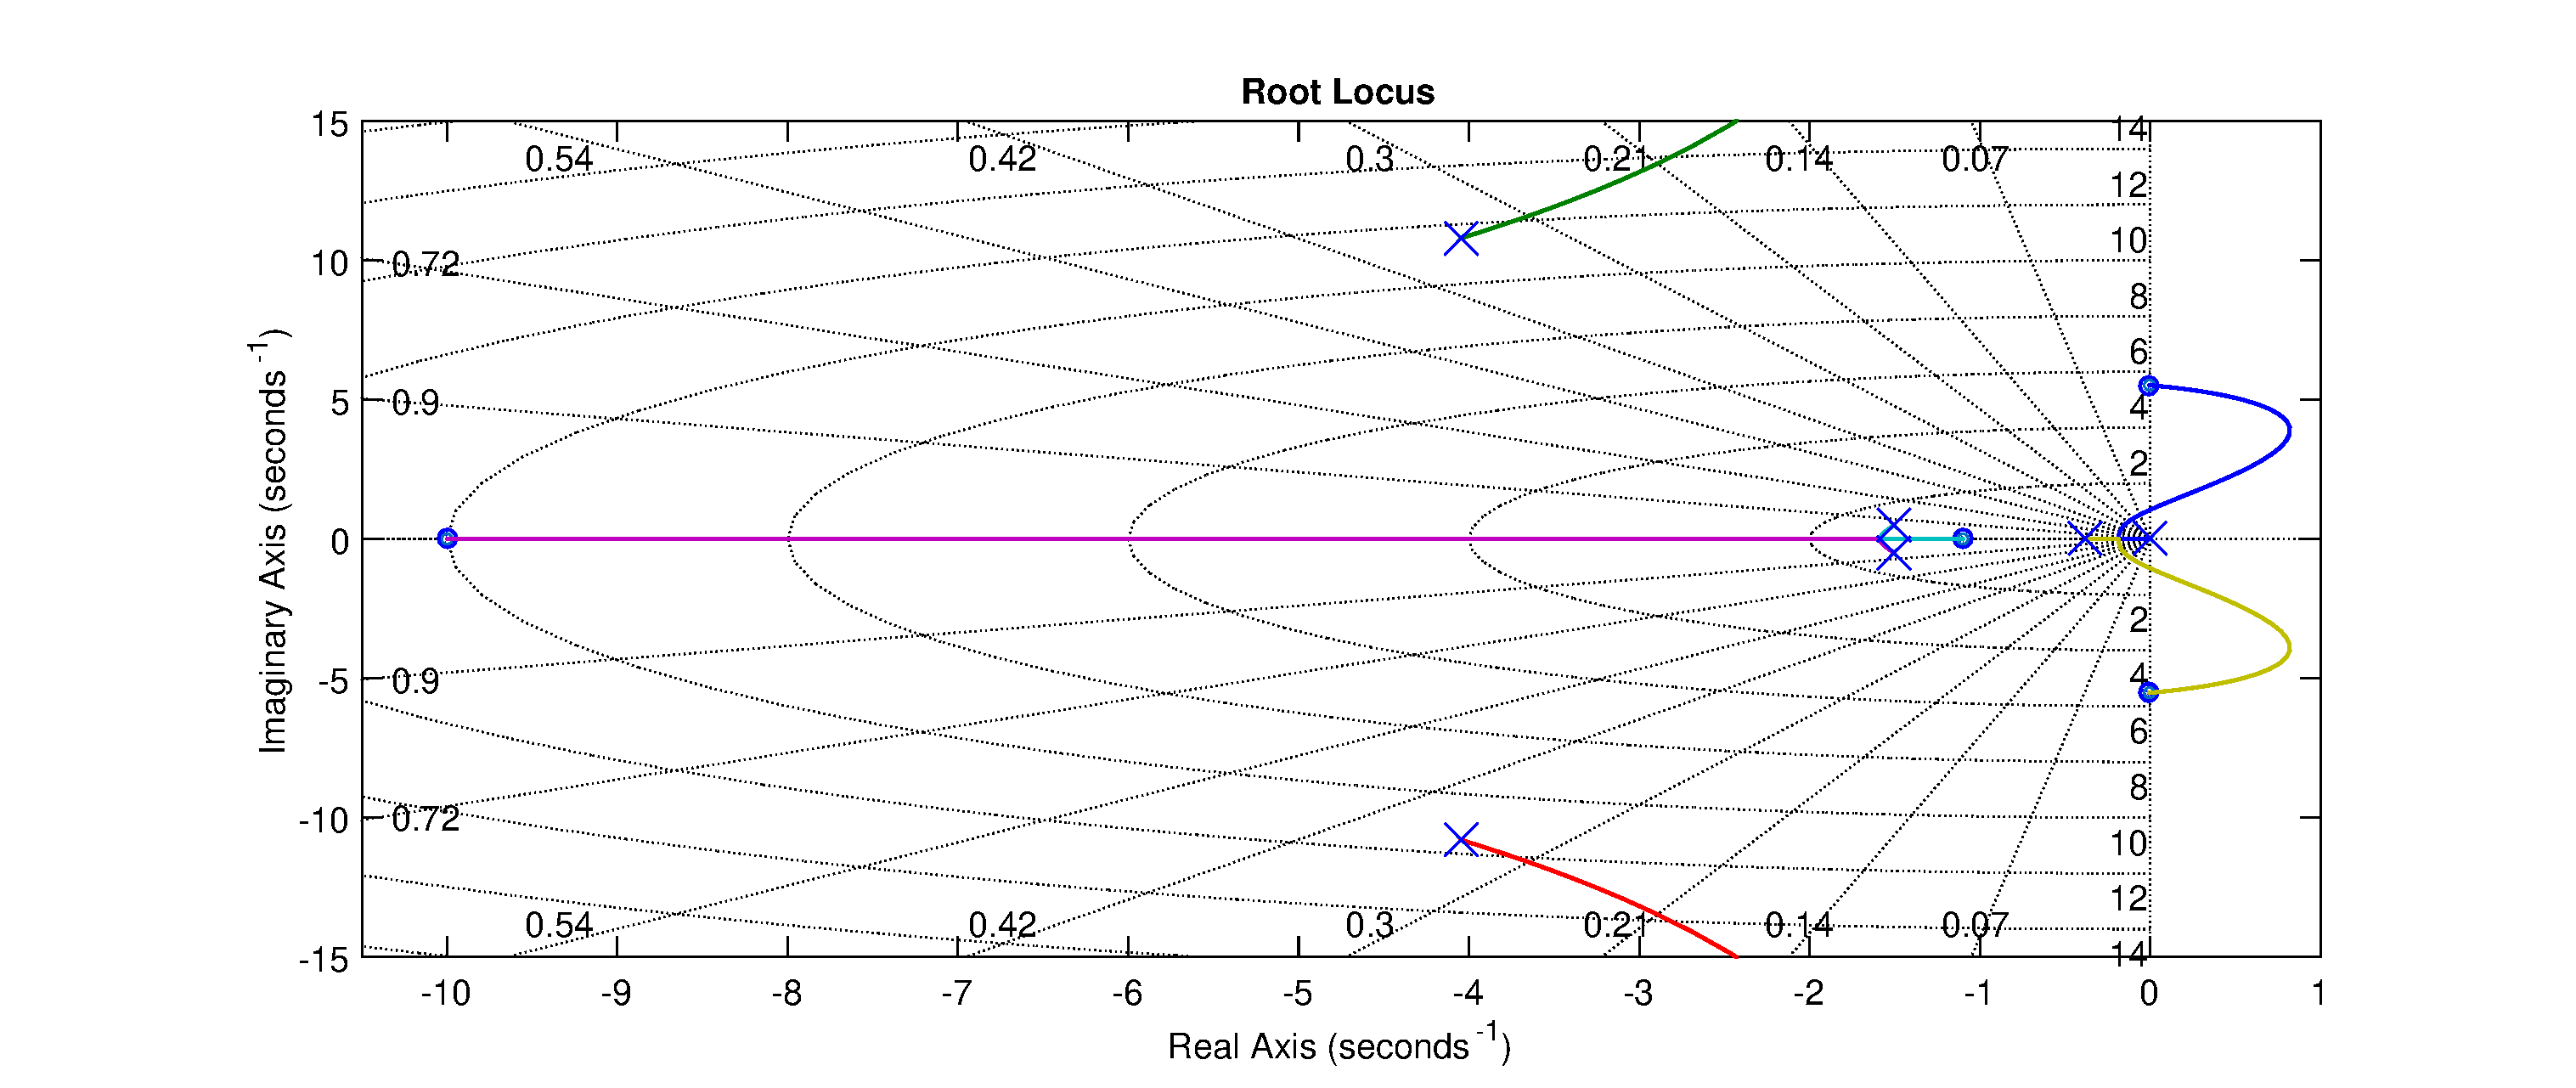
\includegraphics[width=0.9\textwidth]{Billeder/Thomas/Simon}
\end{figure}
\end{frame}

\begin{frame}{Regulatorer}{Root locus trolley}
\vspace{1cm}
\begin{figure}[H]
\centering
\includegraphics[width=0.9\textwidth]{Billeder/Thomas/Trolleyopenloop}
\end{figure}
\end{frame}

\begin{frame}{Regulatorer}{Closed loop step respons trolley}

\begin{figure}[H]
\centering
%\scalebox{0.8} {
% This file was created by matlab2tikz.
%
%The latest updates can be retrieved from
%  http://www.mathworks.com/matlabcentral/fileexchange/22022-matlab2tikz-matlab2tikz
%where you can also make suggestions and rate matlab2tikz.
%
\definecolor{mycolor1}{rgb}{0.00000,0.44700,0.74100}%
%
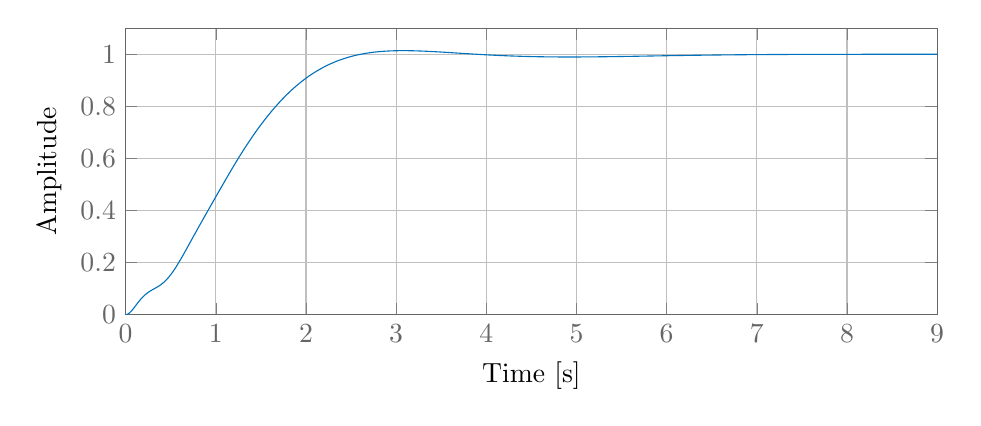
\begin{tikzpicture}

\begin{axis}[%
width=0.85\textwidth,
height=0.3\textwidth,
at={(2.725in,1.103in)},
scale only axis,
separate axis lines,
every outer x axis line/.append style={white!40!black},
every x tick label/.append style={font=\color{white!40!black}},
xmin=0,
xmax=9,
xmajorgrids,
xlabel={Time [s]},
every outer y axis line/.append style={white!40!black},
every y tick label/.append style={font=\color{white!40!black}},
ymin=0,
ymax=1.1,
ymajorgrids,
ytick={0, 0.2, 0.4, 0.6, 0.8, 1, 1.2},
ylabel={Amplitude},
axis background/.style={fill=white}
]
\addplot [color=mycolor1,solid,forget plot]
  table[row sep=crcr]{%
0	0\\
0.00921034037197597	0.000363485735780711\\
0.0184206807439519	0.00140723474645876\\
0.0276310211159279	0.00306069723582055\\
0.0368413614879039	0.00525334333113738\\
0.0460517018598798	0.00791544763283114\\
0.0552620422318558	0.0109788066726706\\
0.0644723826038318	0.0143773859647359\\
0.0736827229758077	0.0180478943895028\\
0.0828930633477837	0.0219302846556475\\
0.0921034037197597	0.0259681795288045\\
0.101313744091736	0.0301092243950357\\
0.110524084463712	0.0343053675339402\\
0.119734424835688	0.0385130702081035\\
0.128944765207664	0.0426934493290905\\
0.13815510557964	0.0468123560336604\\
0.147365445951615	0.0508403939966198\\
0.156575786323591	0.0547528817190136\\
0.165786126695567	0.0585297633633562\\
0.174996467067543	0.062155472963348\\
0.184206807439519	0.0656187570167473\\
0.193417147811495	0.0689124605801913\\
0.202627488183471	0.0720332820277507\\
0.211837828555447	0.0749815016153273\\
0.221048168927423	0.0777606889154993\\
0.230258509299399	0.0803773940572606\\
0.239468849671375	0.0828408275276593\\
0.248679190043351	0.0851625330731555\\
0.257889530415327	0.0873560579832032\\
0.267099870787303	0.0894366247527076\\
0.276310211159279	0.0914208078091819\\
0.285520551531255	0.0933262186600429\\
0.294730891903231	0.0951712024707945\\
0.303941232275207	0.0969745487308874\\
0.313151572647183	0.0987552183055639\\
0.322361913019159	0.100532088813479\\
0.331572253391135	0.102323719915461\\
0.340782593763111	0.104148139753205\\
0.349992934135087	0.106022653441451\\
0.359203274507063	0.107963674196211\\
0.368413614879039	0.109986577377673\\
0.377623955251015	0.112105577441582\\
0.386834295622991	0.114333627529268\\
0.396044635994967	0.116682341185331\\
0.405254976366943	0.119161935474544\\
0.414465316738919	0.121781194576571\\
0.423675657110894	0.124547452768905\\
0.43288599748287	0.127466595565292\\
0.442096337854846	0.130543077658477\\
0.451306678226822	0.133779956222028\\
0.460517018598798	0.137178938055511\\
0.469727358970774	0.140740439009445\\
0.47893769934275	0.144463654100234\\
0.488148039714726	0.14834663671925\\
0.497358380086702	0.152386385353088\\
0.506568720458678	0.156578936262156\\
0.515779060830654	0.160919460610576\\
0.52498940120263	0.165402364600174\\
0.534199741574606	0.170021391233451\\
0.543410081946582	0.174769722412983\\
0.552620422318558	0.179640080176183\\
0.561830762690534	0.184624825962836\\
0.57104110306251	0.189716056916792\\
0.580251443434486	0.194905698331023\\
0.589461783806462	0.200185591455358\\
0.598672124178438	0.205547575997197\\
0.607882464550414	0.210983566756075\\
0.61709280492239	0.216485623941723\\
0.626303145294366	0.222046016831275\\
0.635513485666342	0.227657280523435\\
0.644723826038318	0.233312265644751\\
0.653934166410294	0.239004180955094\\
0.66314450678227	0.244726628885085\\
0.672354847154246	0.250473634117282\\
0.681565187526222	0.256239665394785\\
0.690775527898198	0.262019650805437\\
0.699985868270174	0.267808986846614\\
0.709196208642149	0.273603541624776\\
0.718406549014125	0.279399652585383\\
0.727616889386101	0.285194119202596\\
0.736827229758077	0.290984191084571\\
0.746037570130053	0.29676755196933\\
0.755247910502029	0.302542300098492\\
0.764458250874005	0.308306925461898\\
0.773668591245981	0.314060284405831\\
0.782878931617957	0.319801572091557\\
0.792089271989933	0.325530293279707\\
0.801299612361909	0.331246231900255\\
0.810509952733885	0.336949419847841\\
0.819720293105861	0.342640105418698\\
0.828930633477837	0.348318721778772\\
0.838140973849813	0.353985855823555\\
0.847351314221789	0.359642217758943\\
0.856561654593765	0.365288611699857\\
0.865771994965741	0.370925907549656\\
0.874982335337717	0.376555014389227\\
0.884192675709693	0.382176855570266\\
0.893403016081669	0.387792345673293\\
0.902613356453645	0.393402369457544\\
0.911823696825621	0.399007762897533\\
0.921034037197597	0.404609296369994\\
0.930244377569573	0.410207660025413\\
0.939454717941549	0.415803451350627\\
0.948665058313525	0.42139716490319\\
0.957875398685501	0.426989184174612\\
0.967085739057477	0.432579775518135\\
0.976296079429452	0.43816908405767\\
0.985506419801428	0.443757131477799\\
0.994716760173404	0.44934381558043\\
1.00392710054538	0.454928911481737\\
1.01313744091736	0.460512074313439\\
1.02234778128933	0.466092843285118\\
1.03155812166131	0.471670646959155\\
1.04076846203328	0.477244809586806\\
1.04997880240526	0.482814558352887\\
1.05918914277724	0.488379031377266\\
1.06839948314921	0.49393728632387\\
1.07760982352119	0.499488309471847\\
1.08682016389316	0.505031025108973\\
1.09603050426514	0.510564305113931\\
1.10524084463712	0.516086978601772\\
1.11445118500909	0.521597841515391\\
1.12366152538107	0.527095666055095\\
1.13287186575304	0.53257920984817\\
1.14208220612502	0.538047224770576\\
1.151292546497	0.543498465343369\\
1.16050288686897	0.548931696637056\\
1.16971322724095	0.554345701627698\\
1.17892356761292	0.559739287958994\\
1.1881339079849	0.565111294074834\\
1.19734424835688	0.570460594696646\\
1.20655458872885	0.575786105629322\\
1.21576492910083	0.581086787888421\\
1.2249752694728	0.586361651149718\\
1.23418560984478	0.591609756529875\\
1.24339595021676	0.596830218714094\\
1.25260629058873	0.602022207452925\\
1.26181663096071	0.607184948456073\\
1.27102697133268	0.612317723715919\\
1.28023731170466	0.617419871297621\\
1.28944765207664	0.622490784636099\\
1.29865799244861	0.627529911382912\\
1.30786833282059	0.632536751848041\\
1.31707867319256	0.637510857082944\\
1.32628901356454	0.642451826651961\\
1.33549935393652	0.647359306139257\\
1.34470969430849	0.652232984438066\\
1.35392003468047	0.657072590868057\\
1.36313037505244	0.661877892165225\\
1.37234071542442	0.666648689386927\\
1.3815510557964	0.671384814772511\\
1.39076139616837	0.676086128597488\\
1.39997173654035	0.680752516056519\\
1.40918207691232	0.685383884207508\\
1.4183924172843	0.689980159006031\\
1.42760275765627	0.694541282456147\\
1.43681309802825	0.699067209900334\\
1.44602343840023	0.703557907468052\\
1.4552337787722	0.708013349699158\\
1.46444411914418	0.712433517355179\\
1.47365445951615	0.716818395428332\\
1.48286479988813	0.721167971355186\\
1.49207514026011	0.72548223343897\\
1.50128548063208	0.729761169481865\\
1.51049582100406	0.734004765626076\\
1.51970616137603	0.73821300540018\\
1.52891650174801	0.742385868965144\\
1.53812684211999	0.746523332552512\\
1.54733718249196	0.750625368085619\\
1.55654752286394	0.754691942973233\\
1.56575786323591	0.75872302006387\\
1.57496820360789	0.762718557747988\\
1.58417854397987	0.766678510194574\\
1.59338888435184	0.770602827708033\\
1.60259922472382	0.774491457190988\\
1.61180956509579	0.778344342698427\\
1.62101990546777	0.78216142606866\\
1.63023024583975	0.785942647616758\\
1.63944058621172	0.789687946876465\\
1.6486509265837	0.793397263377088\\
1.65786126695567	0.797070537442431\\
1.66707160732765	0.80070771099958\\
1.67628194769963	0.804308728386132\\
1.6854922880716	0.807873537145295\\
1.69470262844358	0.811402088799272\\
1.70391296881555	0.81489433959226\\
1.71312330918753	0.818350251195407\\
1.72233364955951	0.821769791367093\\
1.73154398993148	0.825152934562896\\
1.74075433030346	0.828499662490619\\
1.74996467067543	0.831809964606744\\
1.75917501104741	0.835083838551599\\
1.76838535141939	0.83832129052149\\
1.77759569179136	0.841522335576867\\
1.78680603216334	0.844686997886435\\
1.79601637253531	0.847815310907869\\
1.80522671290729	0.850907317506478\\
1.81443705327927	0.853963070013796\\
1.82364739365124	0.856982630228636\\
1.83285773402322	0.859966069363608\\
1.84206807439519	0.862913467940553\\
1.85127841476717	0.86582491563866\\
1.86048875513915	0.868700511099319\\
1.86969909551112	0.871540361691983\\
1.8789094358831	0.874344583245442\\
1.88811977625507	0.877113299749\\
1.89733011662705	0.879846643028079\\
1.90654045699903	0.882544752398735\\
1.915750797371	0.885207774305499\\
1.92496113774298	0.887835861946835\\
1.93417147811495	0.890429174892335\\
1.94338181848693	0.892987878695582\\
1.9525921588589	0.895512144506381\\
1.96180249923088	0.898002148685793\\
1.97101283960286	0.900458072427147\\
1.98022317997483	0.9028801013859\\
1.98943352034681	0.905268425320918\\
1.99864386071878	0.907623237749442\\
2.00785420109076	0.909944735617676\\
2.01706454146274	0.912233118988651\\
2.02627488183471	0.914488590748662\\
2.03548522220669	0.916711356333332\\
2.04469556257866	0.91890162347401\\
2.05390590295064	0.921059601964977\\
2.06311624332262	0.923185503451647\\
2.07232658369459	0.9252795412397\\
2.08153692406657	0.927341930124892\\
2.09074726443854	0.929372886243027\\
2.09995760481052	0.931372626939443\\
2.1091679451825	0.933341370657164\\
2.11837828555447	0.935279336842738\\
2.12758862592645	0.937186745868675\\
2.13679896629842	0.939063818971261\\
2.1460093066704	0.940910778202505\\
2.15521964704238	0.942727846394846\\
2.16442998741435	0.944515247137288\\
2.17364032778633	0.946273204761528\\
2.1828506681583	0.948001944336729\\
2.19206100853028	0.94970169167151\\
2.20127134890226	0.951372673321849\\
2.21048168927423	0.953015116603554\\
2.21969202964621	0.954629249608069\\
2.22890237001818	0.956215301220423\\
2.23811271039016	0.957773501138193\\
2.24732305076214	0.959304079890477\\
2.25653339113411	0.960807268855888\\
2.26574373150609	0.962283300278759\\
2.27495407187806	0.963732407282758\\
2.28416441225004	0.965154823881274\\
2.29337475262202	0.966550784984\\
2.30258509299399	0.967920526399231\\
2.31179543336597	0.969264284831517\\
2.32100577373794	0.970582297874371\\
2.33021611410992	0.971874803997842\\
2.3394264544819	0.973142042530841\\
2.34863679485387	0.97438425363818\\
2.35784713522585	0.975601678292371\\
2.36705747559782	0.976794558240285\\
2.3762678159698	0.977963135964848\\
2.38547815634178	0.97910765464199\\
2.39468849671375	0.980228358093119\\
2.40389883708573	0.98132549073344\\
2.4131091774577	0.982399297516461\\
2.42231951782968	0.983450023875064\\
2.43152985820166	0.984477915659535\\
2.44074019857363	0.985483219072971\\
2.44995053894561	0.986466180604485\\
2.45916087931758	0.987427046960631\\
2.46837121968956	0.988366064995481\\
2.47758156006154	0.989283481639765\\
2.48679190043351	0.990179543829486\\
2.49600224080549	0.991054498434402\\
2.50521258117746	0.991908592186752\\
2.51442292154944	0.99274207161057\\
2.52363326192142	0.993555182951938\\
2.53284360229339	0.994348172110448\\
2.54205394266537	0.99512128457219\\
2.55126428303734	0.995874765344477\\
2.56047462340932	0.996608858892544\\
2.56968496378129	0.997323809078413\\
2.57889530415327	0.998019859102059\\
2.58810564452525	0.998697251445035\\
2.59731598489722	0.999356227816627\\
2.6065263252692	0.999997029102631\\
2.61573666564117	1.00061989531678\\
2.62494700601315	1.00122506555488\\
2.63415734638513	1.00181277795152\\
2.6433676867571	1.00238326963958\\
2.65257802712908	1.00293677671217\\
2.66178836750105	1.00347353418725\\
2.67099870787303	1.00399377597455\\
2.68020904824501	1.00449773484493\\
2.68941938861698	1.004985642402\\
2.69862972898896	1.00545772905576\\
2.70784006936093	1.00591422399833\\
2.71705040973291	1.00635535518152\\
2.72626075010489	1.00678134929605\\
2.73547109047686	1.0071924317525\\
2.74468143084884	1.00758882666353\\
2.75389177122081	1.00797075682756\\
2.76310211159279	1.00833844371352\\
2.77231245196477	1.00869210744668\\
2.78152279233674	1.00903196679537\\
2.79073313270872	1.00935823915851\\
2.79994347308069	1.00967114055375\\
2.80915381345267	1.00997088560625\\
2.81836415382465	1.01025768753789\\
2.82757449419662	1.01053175815681\\
2.8367848345686	1.01079330784732\\
2.84599517494057	1.01104254555997\\
2.85520551531255	1.01127967880178\\
2.86441585568453	1.01150491362661\\
2.8736261960565	1.01171845462551\\
2.88283653642848	1.01192050491717\\
2.89204687680045	1.01211126613834\\
2.90125721717243	1.01229093843413\\
2.91046755754441	1.01245972044845\\
2.91967789791638	1.0126178093142\\
2.92888823828836	1.01276540064359\\
2.93809857866033	1.01290268851832\\
2.94730891903231	1.01302986547979\\
2.95651925940429	1.01314712251924\\
2.96572959977626	1.01325464906804\\
2.97493994014824	1.01335263298787\\
2.98415028052021	1.01344126056106\\
2.99336062089219	1.01352071648108\\
3.00257096126417	1.01359118384302\\
3.01178130163614	1.01365284413441\\
3.02099164200812	1.01370587722612\\
3.03020198238009	1.0137504613636\\
3.03941232275207	1.01378677315826\\
3.04862266312405	1.01381498757935\\
3.05783300349602	1.01383527794599\\
3.067043343868	1.01384781591966\\
3.07625368423997	1.01385277149715\\
3.08546402461195	1.01385031300375\\
3.09467436498392	1.01384060708711\\
3.1038847053559	1.0138238187114\\
3.11309504572788	1.013800111152\\
3.12230538609985	1.01376964599078\\
3.13151572647183	1.01373258311176\\
3.1407260668438	1.0136890806974\\
3.14993640721578	1.01363929522535\\
3.15914674758776	1.0135833814658\\
3.16835708795973	1.01352149247933\\
3.17756742833171	1.01345377961531\\
3.18677776870368	1.01338039251081\\
3.19598810907566	1.01330147909011\\
3.20519844944764	1.01321718556462\\
3.21440878981961	1.01312765643344\\
3.22361913019159	1.0130330344843\\
3.23282947056356	1.01293346079508\\
3.24203981093554	1.01282907473574\\
3.25125015130752	1.01272001397076\\
3.26046049167949	1.01260641446197\\
3.26967083205147	1.01248841047182\\
3.27888117242344	1.01236613456713\\
3.28809151279542	1.01223971762308\\
3.2973018531674	1.01210928882769\\
3.30651219353937	1.01197497568663\\
3.31572253391135	1.0118369040283\\
3.32493287428332	1.01169519800933\\
3.3341432146553	1.01154998012025\\
3.34335355502728	1.01140137119157\\
3.35256389539925	1.01124949040001\\
3.36177423577123	1.01109445527505\\
3.3709845761432	1.01093638170567\\
3.38019491651518	1.01077538394736\\
3.38940525688716	1.01061157462924\\
3.39861559725913	1.0104450647615\\
3.40782593763111	1.01027596374286\\
3.41703627800308	1.01010437936837\\
3.42624661837506	1.00993041783722\\
3.43545695874704	1.0097541837608\\
3.44466729911901	1.00957578017084\\
3.45387763949099	1.00939530852773\\
3.46308797986296	1.00921286872891\\
3.47229832023494	1.00902855911746\\
3.48150866060692	1.00884247649072\\
3.49071900097889	1.00865471610911\\
3.49992934135087	1.00846537170498\\
3.50913968172284	1.00827453549164\\
3.51835002209482	1.0080822981724\\
3.5275603624668	1.00788874894984\\
3.53677070283877	1.00769397553506\\
3.54598104321075	1.00749806415711\\
3.55519138358272	1.00730109957248\\
3.5644017239547	1.00710316507467\\
3.57361206432667	1.00690434250395\\
3.58282240469865	1.00670471225709\\
3.59203274507063	1.00650435329728\\
3.6012430854426	1.00630334316413\\
3.61045342581458	1.00610175798371\\
3.61966376618655	1.00589967247878\\
3.62887410655853	1.00569715997904\\
3.63808444693051	1.00549429243148\\
3.64729478730248	1.00529114041088\\
3.65650512767446	1.00508777313037\\
3.66571546804643	1.00488425845203\\
3.67492580841841	1.0046806628977\\
3.68413614879039	1.00447705165973\\
3.69334648916236	1.00427348861199\\
3.70255682953434	1.00407003632077\\
3.71176716990631	1.00386675605597\\
3.72097751027829	1.00366370780217\\
3.73018785065027	1.00346095026993\\
3.73939819102224	1.00325854090712\\
3.74860853139422	1.00305653591025\\
3.75781887176619	1.002854990236\\
3.76702921213817	1.00265395761268\\
3.77623955251015	1.00245349055188\\
3.78544989288212	1.00225364036007\\
3.7946602332541	1.00205445715031\\
3.80387057362607	1.00185598985403\\
3.81308091399805	1.00165828623277\\
3.82229125437003	1.00146139289006\\
3.831501594742	1.00126535528331\\
3.84071193511398	1.00107021773567\\
3.84992227548595	1.00087602344804\\
3.85913261585793	1.00068281451097\\
3.86834295622991	1.00049063191669\\
3.87755329660188	1.00029951557114\\
3.88676363697386	1.00010950430595\\
3.89597397734583	0.99992063589049\\
3.90518431771781	0.999732947043924\\
3.91439465808979	0.999546473447249\\
3.92360499846176	0.999361249755336\\
3.93281533883374	0.999177309608974\\
3.94202567920571	0.998994685646907\\
3.95123601957769	0.998813409517855\\
3.96044635994967	0.998633511892525\\
3.96965670032164	0.99845502247561\\
3.97886704069362	0.99827797001776\\
3.98807738106559	0.998102382327539\\
3.99728772143757	0.997928286283355\\
4.00649806180955	0.997755707845364\\
4.01570840218152	0.997584672067342\\
4.0249187425535	0.99741520310853\\
4.03412908292547	0.997247324245446\\
4.04333942329745	0.997081057883656\\
4.05254976366943	0.996916425569514\\
4.0617601040414	0.996753448001862\\
4.07097044441338	0.996592145043687\\
4.08018078478535	0.996432535733739\\
4.08939112515733	0.996274638298102\\
4.09860146552931	0.996118470161724\\
4.10781180590128	0.995964047959894\\
4.11702214627326	0.995811387549685\\
4.12623248664523	0.995660504021328\\
4.13544282701721	0.995511411709556\\
4.14465316738919	0.995364124204882\\
4.15386350776116	0.995218654364832\\
4.16307384813314	0.995075014325124\\
4.17228418850511	0.99493321551079\\
4.18149452887709	0.994793268647242\\
4.19070486924906	0.994655183771289\\
4.19991520962104	0.994518970242084\\
4.20912554999302	0.994384636752024\\
4.21833589036499	0.994252191337587\\
4.22754623073697	0.994121641390103\\
4.23675657110894	0.993992993666471\\
4.24596691148092	0.993866254299814\\
4.2551772518529	0.993741428810063\\
4.26438759222487	0.99361852211449\\
4.27359793259685	0.993497538538158\\
4.28280827296882	0.993378481824327\\
4.2920186133408	0.993261355144775\\
4.30122895371278	0.993146161110058\\
4.31043929408475	0.99303290177971\\
4.31964963445673	0.992921578672357\\
4.3288599748287	0.992812192775777\\
4.33807031520068	0.992704744556875\\
4.34728065557266	0.992599233971602\\
4.35649099594463	0.992495660474786\\
4.36570133631661	0.9923940230299\\
4.37491167668858	0.992294320118749\\
4.38412201706056	0.99219654975109\\
4.39333235743254	0.992100709474169\\
4.40254269780451	0.992006796382183\\
4.41175303817649	0.99191480712567\\
4.42096337854846	0.991824737920818\\
4.43017371892044	0.991736584558689\\
4.43938405929242	0.991650342414378\\
4.44859439966439	0.991566006456082\\
4.45780474003637	0.991483571254088\\
4.46701508040834	0.991403030989689\\
4.47622542078032	0.991324379464014\\
4.4854357611523	0.99124761010677\\
4.49464610152427	0.991172715984912\\
4.50385644189625	0.991099689811228\\
4.51306678226822	0.991028523952833\\
4.5222771226402	0.990959210439596\\
4.53148746301218	0.990891740972461\\
4.54069780338415	0.990826106931706\\
4.54990814375613	0.990762299385104\\
4.5591184841281	0.990700309096004\\
4.56832882450008	0.990640126531328\\
4.57753916487206	0.99058174186948\\
4.58674950524403	0.990525145008174\\
4.59595984561601	0.990470325572174\\
4.60517018598798	0.990417272920952\\
4.61438052635996	0.990365976156253\\
4.62359086673194	0.990316424129587\\
4.63280120710391	0.990268605449622\\
4.64201154747589	0.990222508489503\\
4.65122188784786	0.990178121394078\\
4.66043222821984	0.990135432087043\\
4.66964256859182	0.990094428278\\
4.67885290896379	0.990055097469428\\
4.68806324933577	0.990017426963574\\
4.69727358970774	0.989981403869255\\
4.70648393007972	0.989947015108574\\
4.71569427045169	0.989914247423556\\
4.72490461082367	0.989883087382695\\
4.73411495119565	0.98985352138742\\
4.74332529156762	0.989825535678473\\
4.7525356319396	0.98979911634221\\
4.76174597231157	0.989774249316806\\
4.77095631268355	0.989750920398393\\
4.78016665305553	0.989729115247101\\
4.7893769934275	0.989708819393018\\
4.79858733379948	0.989690018242079\\
4.80779767417145	0.989672697081856\\
4.81700801454343	0.989656841087275\\
4.82621835491541	0.989642435326254\\
4.83542869528738	0.989629464765251\\
4.84463903565936	0.989617914274737\\
4.85384937603133	0.989607768634584\\
4.86305971640331	0.989599012539379\\
4.87227005677529	0.989591630603647\\
4.88148039714726	0.989585607367008\\
4.89069073751924	0.989580927299239\\
4.89990107789121	0.989577574805274\\
4.90911141826319	0.989575534230107\\
4.91832175863517	0.989574789863632\\
4.92753209900714	0.989575325945398\\
4.93674243937912	0.989577126669283\\
4.94595277975109	0.989580176188103\\
4.95516312012307	0.989584458618127\\
4.96437346049505	0.989589958043535\\
4.97358380086702	0.989596658520783\\
4.982794141239	0.989604544082901\\
4.99200448161097	0.989613598743718\\
5.00121482198295	0.989623806502009\\
5.01042516235493	0.989635151345564\\
5.0196355027269	0.989647617255192\\
5.02884584309888	0.989661188208648\\
5.03805618347085	0.989675848184485\\
5.04726652384283	0.989691581165834\\
5.05647686421481	0.98970837114412\\
5.06568720458678	0.989726202122699\\
5.07489754495876	0.989745058120423\\
5.08410788533073	0.989764923175144\\
5.09331822570271	0.989785781347138\\
5.10252856607469	0.989807616722473\\
5.11173890644666	0.989830413416288\\
5.12094924681864	0.989854155576032\\
5.13015958719061	0.989878827384605\\
5.13936992756259	0.98990441306346\\
5.14858026793457	0.989930896875618\\
5.15779060830654	0.989958263128629\\
5.16700094867852	0.989986496177465\\
5.17621128905049	0.990015580427343\\
5.18542162942247	0.990045500336496\\
5.19463196979445	0.990076240418866\\
5.20384231016642	0.990107785246747\\
5.2130526505384	0.990140119453357\\
5.22226299091037	0.990173227735351\\
5.23147333128235	0.990207094855279\\
5.24068367165432	0.99024170564397\\
5.2498940120263	0.990277045002869\\
5.25910435239828	0.99031309790631\\
5.26831469277025	0.990349849403727\\
5.27752503314223	0.990387284621812\\
5.2867353735142	0.990425388766616\\
5.29594571388618	0.990464147125585\\
5.30515605425816	0.99050354506955\\
5.31436639463013	0.990543568054653\\
5.32357673500211	0.990584201624226\\
5.33278707537408	0.990625431410608\\
5.34199741574606	0.990667243136911\\
5.35120775611804	0.990709622618735\\
5.36041809649001	0.990752555765829\\
5.36962843686199	0.990796028583697\\
5.37883877723396	0.990840027175154\\
5.38804911760594	0.990884537741836\\
5.39725945797792	0.990929546585657\\
5.40646979834989	0.990975040110208\\
5.41568013872187	0.991021004822121\\
5.42489047909384	0.991067427332377\\
5.43410081946582	0.991114294357566\\
5.4433111598378	0.991161592721101\\
5.45252150020977	0.991209309354386\\
5.46173184058175	0.991257431297938\\
5.47094218095372	0.991305945702463\\
5.4801525213257	0.991354839829887\\
5.48936286169768	0.991404101054343\\
5.49857320206965	0.991453716863117\\
5.50778354244163	0.991503674857546\\
5.5169938828136	0.991553962753876\\
5.52620422318558	0.991604568384081\\
5.53541456355756	0.991655479696637\\
5.54462490392953	0.991706684757257\\
5.55383524430151	0.991758171749585\\
5.56304558467348	0.991809928975853\\
5.57225592504546	0.991861944857494\\
5.58146626541744	0.991914207935723\\
5.59067660578941	0.991966706872078\\
5.59988694616139	0.992019430448919\\
5.60909728653336	0.9920723675699\\
5.61830762690534	0.992125507260393\\
5.62751796727732	0.992178838667891\\
5.63672830764929	0.992232351062363\\
5.64593864802127	0.99228603383658\\
5.65514898839324	0.99233987650641\\
5.66435932876522	0.992393868711075\\
5.6735696691372	0.992448000213378\\
5.68278000950917	0.992502260899899\\
5.69199034988115	0.992556640781152\\
5.70120069025312	0.992611129991726\\
5.7104110306251	0.992665718790376\\
5.71962137099707	0.992720397560102\\
5.72883171136905	0.992775156808188\\
5.73804205174103	0.992829987166216\\
5.747252392113	0.992884879390047\\
5.75646273248498	0.992939824359786\\
5.76567307285695	0.992994813079701\\
5.77488341322893	0.993049836678136\\
5.78409375360091	0.993104886407379\\
5.79330409397288	0.99315995364352\\
5.80251443434486	0.993215029886271\\
5.81172477471683	0.993270106758771\\
5.82093511508881	0.993325176007359\\
5.83014545546079	0.993380229501328\\
5.83935579583276	0.993435259232655\\
5.84856613620474	0.99349025731571\\
5.85777647657671	0.993545215986934\\
5.86698681694869	0.993600127604509\\
5.87619715732067	0.993654984647992\\
5.88540749769264	0.993709779717942\\
5.89461783806462	0.993764505535516\\
5.90382817843659	0.99381915494205\\
5.91303851880857	0.993873720898619\\
5.92224885918055	0.993928196485579\\
5.93145919955252	0.99398257490209\\
5.9406695399245	0.994036849465619\\
5.94987988029647	0.994091013611431\\
5.95909022066845	0.994145060892054\\
5.96830056104043	0.994198984976734\\
5.9775109014124	0.994252779650873\\
5.98672124178438	0.994306438815446\\
5.99593158215635	0.994359956486409\\
6.00514192252833	0.994413326794088\\
6.01435226290031	0.994466543982552\\
6.02356260327228	0.994519602408977\\
6.03277294364426	0.994572496542991\\
6.04198328401623	0.994625220966007\\
6.05119362438821	0.994677770370544\\
6.06040396476019	0.994730139559535\\
6.06961430513216	0.994782323445618\\
6.07882464550414	0.994834317050424\\
6.08803498587611	0.994886115503848\\
6.09724532624809	0.994937714043305\\
6.10645566662007	0.994989108012983\\
6.11566600699204	0.995040292863081\\
6.12487634736402	0.995091264149039\\
6.13408668773599	0.995142017530752\\
6.14329702810797	0.995192548771787\\
6.15250736847995	0.995242853738577\\
6.16171770885192	0.995292928399616\\
6.1709280492239	0.99534276882464\\
6.18013838959587	0.995392371183804\\
6.18934872996785	0.995441731746851\\
6.19855907033983	0.995490846882266\\
6.2077694107118	0.995539713056437\\
6.21697975108378	0.995588326832793\\
6.22619009145575	0.99563668487095\\
6.23540043182773	0.99568478392584\\
6.24461077219971	0.995732620846843\\
6.25382111257168	0.995780192576904\\
6.26303145294366	0.995827496151654\\
6.27224179331563	0.995874528698518\\
6.28145213368761	0.995921287435828\\
6.29066247405959	0.995967769671917\\
6.29987281443156	0.996013972804227\\
6.30908315480354	0.996059894318394\\
6.31829349517551	0.996105531787349\\
6.32750383554749	0.996150882870398\\
6.33671417591947	0.99619594531231\\
6.34592451629144	0.996240716942398\\
6.35513485666342	0.9962851956736\\
6.36434519703539	0.996329379501553\\
6.37355553740737	0.996373266503672\\
6.38276587777935	0.996416854838219\\
6.39197621815132	0.996460142743377\\
6.4011865585233	0.996503128536319\\
6.41039689889527	0.99654581061228\\
6.41960723926725	0.996588187443619\\
6.42881757963923	0.996630257578894\\
6.4380279200112	0.996672019641924\\
6.44723826038318	0.996713472330858\\
6.45644860075515	0.99675461441724\\
6.46565894112713	0.996795444745078\\
6.4748692814991	0.996835962229912\\
6.48407962187108	0.996876165857879\\
6.49328996224306	0.996916054684781\\
6.50250030261503	0.996955627835161\\
6.51171064298701	0.996994884501367\\
6.52092098335898	0.997033823942628\\
6.53013132373096	0.997072445484126\\
6.53934166410294	0.997110748516072\\
6.54855200447491	0.997148732492783\\
6.55776234484689	0.997186396931761\\
6.56697268521886	0.997223741412777\\
6.57618302559084	0.997260765576949\\
6.58539336596282	0.997297469125835\\
6.59460370633479	0.997333851820517\\
6.60381404670677	0.997369913480697\\
6.61302438707874	0.997405653983788\\
6.62223472745072	0.997441073264014\\
6.6314450678227	0.997476171311509\\
6.64065540819467	0.997510948171428\\
6.64986574856665	0.997545403943046\\
6.65907608893862	0.997579538778877\\
6.6682864293106	0.997613352883787\\
6.67749676968258	0.99764684651411\\
6.68670711005455	0.997680019976781\\
6.69591745042653	0.997712873628454\\
6.7051277907985	0.997745407874637\\
6.71433813117048	0.997777623168834\\
6.72354847154246	0.997809520011677\\
6.73275881191443	0.997841098950078\\
6.74196915228641	0.997872360576377\\
6.75117949265838	0.997903305527498\\
6.76038983303036	0.997933934484106\\
6.76960017340234	0.997964248169778\\
6.77881051377431	0.997994247350168\\
6.78802085414629	0.998023932832182\\
6.79723119451826	0.998053305463165\\
6.80644153489024	0.998082366130079\\
6.81565187526222	0.9981111157587\\
6.82486221563419	0.998139555312814\\
6.83407255600617	0.998167685793418\\
6.84328289637814	0.998195508237929\\
6.85249323675012	0.998223023719399\\
6.8617035771221	0.998250233345734\\
6.87091391749407	0.998277138258921\\
6.88012425786605	0.998303739634257\\
6.88933459823802	0.998330038679592\\
6.89854493861	0.998356036634566\\
6.90775527898198	0.998381734769865\\
6.91696561935395	0.998407134386475\\
6.92617595972593	0.998432236814942\\
6.9353863000979	0.998457043414646\\
6.94459664046988	0.99848155557307\\
6.95380698084186	0.998505774705089\\
6.96301732121383	0.998529702252249\\
6.97222766158581	0.998553339682068\\
6.98143800195778	0.998576688487336\\
6.99064834232976	0.998599750185419\\
6.99985868270173	0.998622526317576\\
7.00906902307371	0.998645018448281\\
7.01827936344569	0.998667228164543\\
7.02748970381766	0.998689157075252\\
7.03670004418964	0.998710806810506\\
7.04591038456161	0.99873217902097\\
7.05512072493359	0.998753275377224\\
7.06433106530557	0.998774097569124\\
7.07354140567754	0.998794647305171\\
7.08275174604952	0.998814926311886\\
7.09196208642149	0.99883493633319\\
7.10117242679347	0.998854679129795\\
7.11038276716545	0.998874156478592\\
7.11959310753742	0.998893370172061\\
7.1288034479094	0.998912322017676\\
7.13801378828137	0.998931013837319\\
7.14722412865335	0.998949447466707\\
7.15643446902533	0.998967624754815\\
7.1656448093973	0.998985547563318\\
7.17485514976928	0.999003217766032\\
7.18406549014125	0.999020637248363\\
7.19327583051323	0.999037807906764\\
7.20248617088521	0.999054731648199\\
7.21169651125718	0.999071410389617\\
7.22090685162916	0.999087846057423\\
7.23011719200113	0.999104040586968\\
7.23932753237311	0.999119995922035\\
7.24853787274509	0.999135714014342\\
7.25774821311706	0.999151196823046\\
7.26695855348904	0.999166446314249\\
7.27616889386101	0.999181464460526\\
7.28537923423299	0.999196253240439\\
7.29458957460497	0.999210814638081\\
7.30379991497694	0.999225150642603\\
7.31301025534892	0.99923926324777\\
7.32222059572089	0.999253154451503\\
7.33143093609287	0.999266826255448\\
7.34064127646485	0.999280280664534\\
7.34985161683682	0.999293519686548\\
7.3590619572088	0.999306545331712\\
7.36827229758077	0.999319359612272\\
7.37748263795275	0.999331964542087\\
7.38669297832473	0.999344362136227\\
7.3959033186967	0.999356554410581\\
7.40511365906868	0.999368543381464\\
7.41432399944065	0.999380331065238\\
7.42353433981263	0.999391919477938\\
7.43274468018461	0.999403310634896\\
7.44195502055658	0.999414506550386\\
7.45116536092856	0.999425509237262\\
7.46037570130053	0.99943632070661\\
7.46958604167251	0.999446942967401\\
7.47879638204448	0.999457378026158\\
7.48800672241646	0.99946762788662\\
7.49721706278844	0.999477694549418\\
7.50642740316041	0.999487580011755\\
7.51563774353239	0.999497286267094\\
7.52484808390436	0.99950681530485\\
7.53405842427634	0.999516169110085\\
7.54326876464832	0.999525349663219\\
7.55247910502029	0.999534358939737\\
7.56168944539227	0.999543198909903\\
7.57089978576424	0.999551871538487\\
7.58011012613622	0.99956037878449\\
7.5893204665082	0.999568722600875\\
7.59853080688017	0.999576904934315\\
7.60774114725215	0.999584927724928\\
7.61695148762412	0.999592792906034\\
7.6261618279961	0.999600502403908\\
7.63537216836808	0.999608058137545\\
7.64458250874005	0.999615462018422\\
7.65379284911203	0.999622715950276\\
7.663003189484	0.999629821828879\\
7.67221352985598	0.99963678154182\\
7.68142387022796	0.999643596968297\\
7.69063421059993	0.99965026997891\\
7.69984455097191	0.999656802435457\\
7.70905489134388	0.999663196190742\\
7.71826523171586	0.999669453088381\\
7.72747557208784	0.999675574962618\\
7.73668591245981	0.999681563638146\\
7.74589625283179	0.999687420929927\\
7.75510659320376	0.999693148643024\\
7.76431693357574	0.999698748572436\\
7.77352727394772	0.999704222502932\\
7.78273761431969	0.9997095722089\\
7.79194795469167	0.999714799454192\\
7.80115829506364	0.99971990599198\\
7.81036863543562	0.999724893564608\\
7.8195789758076	0.99972976390346\\
7.82878931617957	0.999734518728822\\
7.83799965655155	0.999739159749757\\
7.84720999692352	0.999743688663976\\
7.8564203372955	0.999748107157724\\
7.86563067766748	0.999752416905656\\
7.87484101803945	0.999756619570731\\
7.88405135841143	0.999760716804106\\
7.8932616987834	0.999764710245025\\
7.90247203915538	0.999768601520729\\
7.91168237952736	0.999772392246354\\
7.92089271989933	0.999776084024843\\
7.93010306027131	0.999779678446859\\
7.93931340064328	0.999783177090699\\
7.94852374101526	0.999786581522218\\
7.95773408138724	0.999789893294752\\
7.96694442175921	0.999793113949045\\
7.97615476213119	0.999796245013182\\
7.98536510250316	0.999799288002526\\
7.99457544287514	0.999802244419652\\
8.00378578324712	0.999805115754296\\
8.01299612361909	0.999807903483296\\
8.02220646399107	0.999810609070546\\
8.03141680436304	0.999813233966945\\
8.04062714473502	0.999815779610356\\
8.04983748510699	0.999818247425563\\
8.05904782547897	0.999820638824239\\
8.06825816585095	0.999822955204906\\
8.07746850622292	0.999825197952908\\
8.0866788465949	0.999827368440382\\
8.09588918696688	0.999829468026236\\
8.10509952733885	0.999831498056124\\
8.11430986771083	0.999833459862429\\
8.1235202080828	0.999835354764248\\
8.13273054845478	0.999837184067377\\
8.14194088882675	0.999838949064306\\
8.15115122919873	0.999840651034205\\
8.16036156957071	0.999842291242927\\
8.16957190994268	0.999843870942999\\
8.17878225031466	0.999845391373629\\
8.18799259068664	0.999846853760706\\
8.19720293105861	0.999848259316807\\
8.20641327143059	0.999849609241207\\
8.21562361180256	0.999850904719886\\
8.22483395217454	0.99985214692555\\
8.23404429254651	0.999853337017637\\
8.24325463291849	0.999854476142344\\
8.25246497329047	0.999855565432642\\
8.26167531366244	0.999856606008302\\
8.27088565403442	0.999857598975916\\
8.28009599440639	0.999858545428928\\
8.28930633477837	0.999859446447662\\
8.29851667515035	0.999860303099352\\
8.30772701552232	0.999861116438177\\
8.3169373558943	0.999861887505294\\
8.32614769626627	0.999862617328877\\
8.33535803663825	0.999863306924157\\
8.34456837701023	0.99986395729346\\
8.3537787173822	0.999864569426252\\
8.36298905775418	0.999865144299181\\
8.37219939812615	0.999865682876129\\
8.38140973849813	0.999866186108252\\
8.39062007887011	0.999866654934038\\
8.39983041924208	0.99986709027935\\
8.40904075961406	0.999867493057486\\
8.41825109998603	0.999867864169228\\
8.42746144035801	0.999868204502903\\
8.43667178072999	0.999868514934434\\
8.44588212110196	0.999868796327406\\
8.45509246147394	0.999869049533121\\
8.46430280184591	0.999869275390661\\
8.47351314221789	0.999869474726952\\
8.48272348258987	0.999869648356826\\
8.49193382296184	0.999869797083089\\
8.50114416333382	0.999869921696586\\
8.51035450370579	0.999870022976269\\
8.51956484407777	0.999870101689267\\
8.52877518444975	0.999870158590953\\
8.53798552482172	0.999870194425022\\
8.5471958651937	0.999870209923553\\
8.55640620556567	0.999870205807093\\
8.56561654593765	0.999870182784722\\
8.57482688630962	0.999870141554137\\
8.5840372266816	0.999870082801719\\
8.59324756705358	0.999870007202617\\
8.60245790742555	0.999869915420822\\
8.61166824779753	0.999869808109248\\
8.62087858816951	0.99986968590981\\
8.63008892854148	0.999869549453505\\
8.63929926891346	0.99986939936049\\
8.64850960928543	0.999869236240171\\
8.65771994965741	0.999869060691276\\
8.66693029002938	0.999868873301945\\
8.67614063040136	0.99986867464981\\
8.68535097077334	0.999868465302082\\
8.69456131114531	0.999868245815633\\
8.70377165151729	0.999868016737082\\
8.71298199188927	0.999867778602882\\
8.72219233226124	0.999867531939406\\
8.73140267263322	0.999867277263031\\
8.74061301300519	0.999867015080231\\
8.74982335337717	0.999866745887658\\
8.75903369374914	0.999866470172236\\
8.76824403412112	0.999866188411243\\
8.7774543744931	0.999865901072407\\
8.78666471486507	0.999865608613988\\
8.79587505523705	0.999865311484871\\
8.80508539560902	0.999865010124657\\
8.814295735981	0.999864704963749\\
8.82350607635298	0.999864396423443\\
8.83271641672495	0.999864084916021\\
8.84192675709693	0.999863770844839\\
8.8511370974689	0.999863454604415\\
8.86034743784088	0.999863136580527\\
8.86955777821286	0.999862817150295\\
8.87876811858483	0.99986249668228\\
8.88797845895681	0.999862175536568\\
8.89718879932878	0.999861854064866\\
8.90639913970076	0.999861532610591\\
8.91560948007274	0.99986121150896\\
8.92481982044471	0.999860891087083\\
8.93403016081669	0.999860571664054\\
8.94324050118866	0.999860253551039\\
8.95245084156064	0.999859937051371\\
8.96166118193262	0.999859622460639\\
8.97087152230459	0.999859310066777\\
8.98008186267657	0.999859000150158\\
8.98929220304854	0.999858692983681\\
8.99850254342052	0.999858388832866\\
9.00771288379249	0.999858087955939\\
};
\end{axis}
\end{tikzpicture}%
%}
%\includegraphics[width=1.1\textwidth]{Billeder/Thomas/cl_x_step}
\end{figure}


\vspace{0.2cm}
\begin{description}
    \item[\textbf{(E)}] : x-akse settling time, $t_s \leq 17,45 s$
    \item[\textbf{(F)}] : x-akse steady-state-error, $e_{ss} = 0,0\%$ 
    \item[\textbf{(G)}] : x-akse overshoot, $M_p \leq 6,4\%$
\end{description}
\vspace{0.6cm}

\end{frame}

\begin{frame}{Regulatorer}{Simulering af closed loop med statisk friktion kompensering}
\vspace{1.5cm}
\begin{figure}[H]
\centering
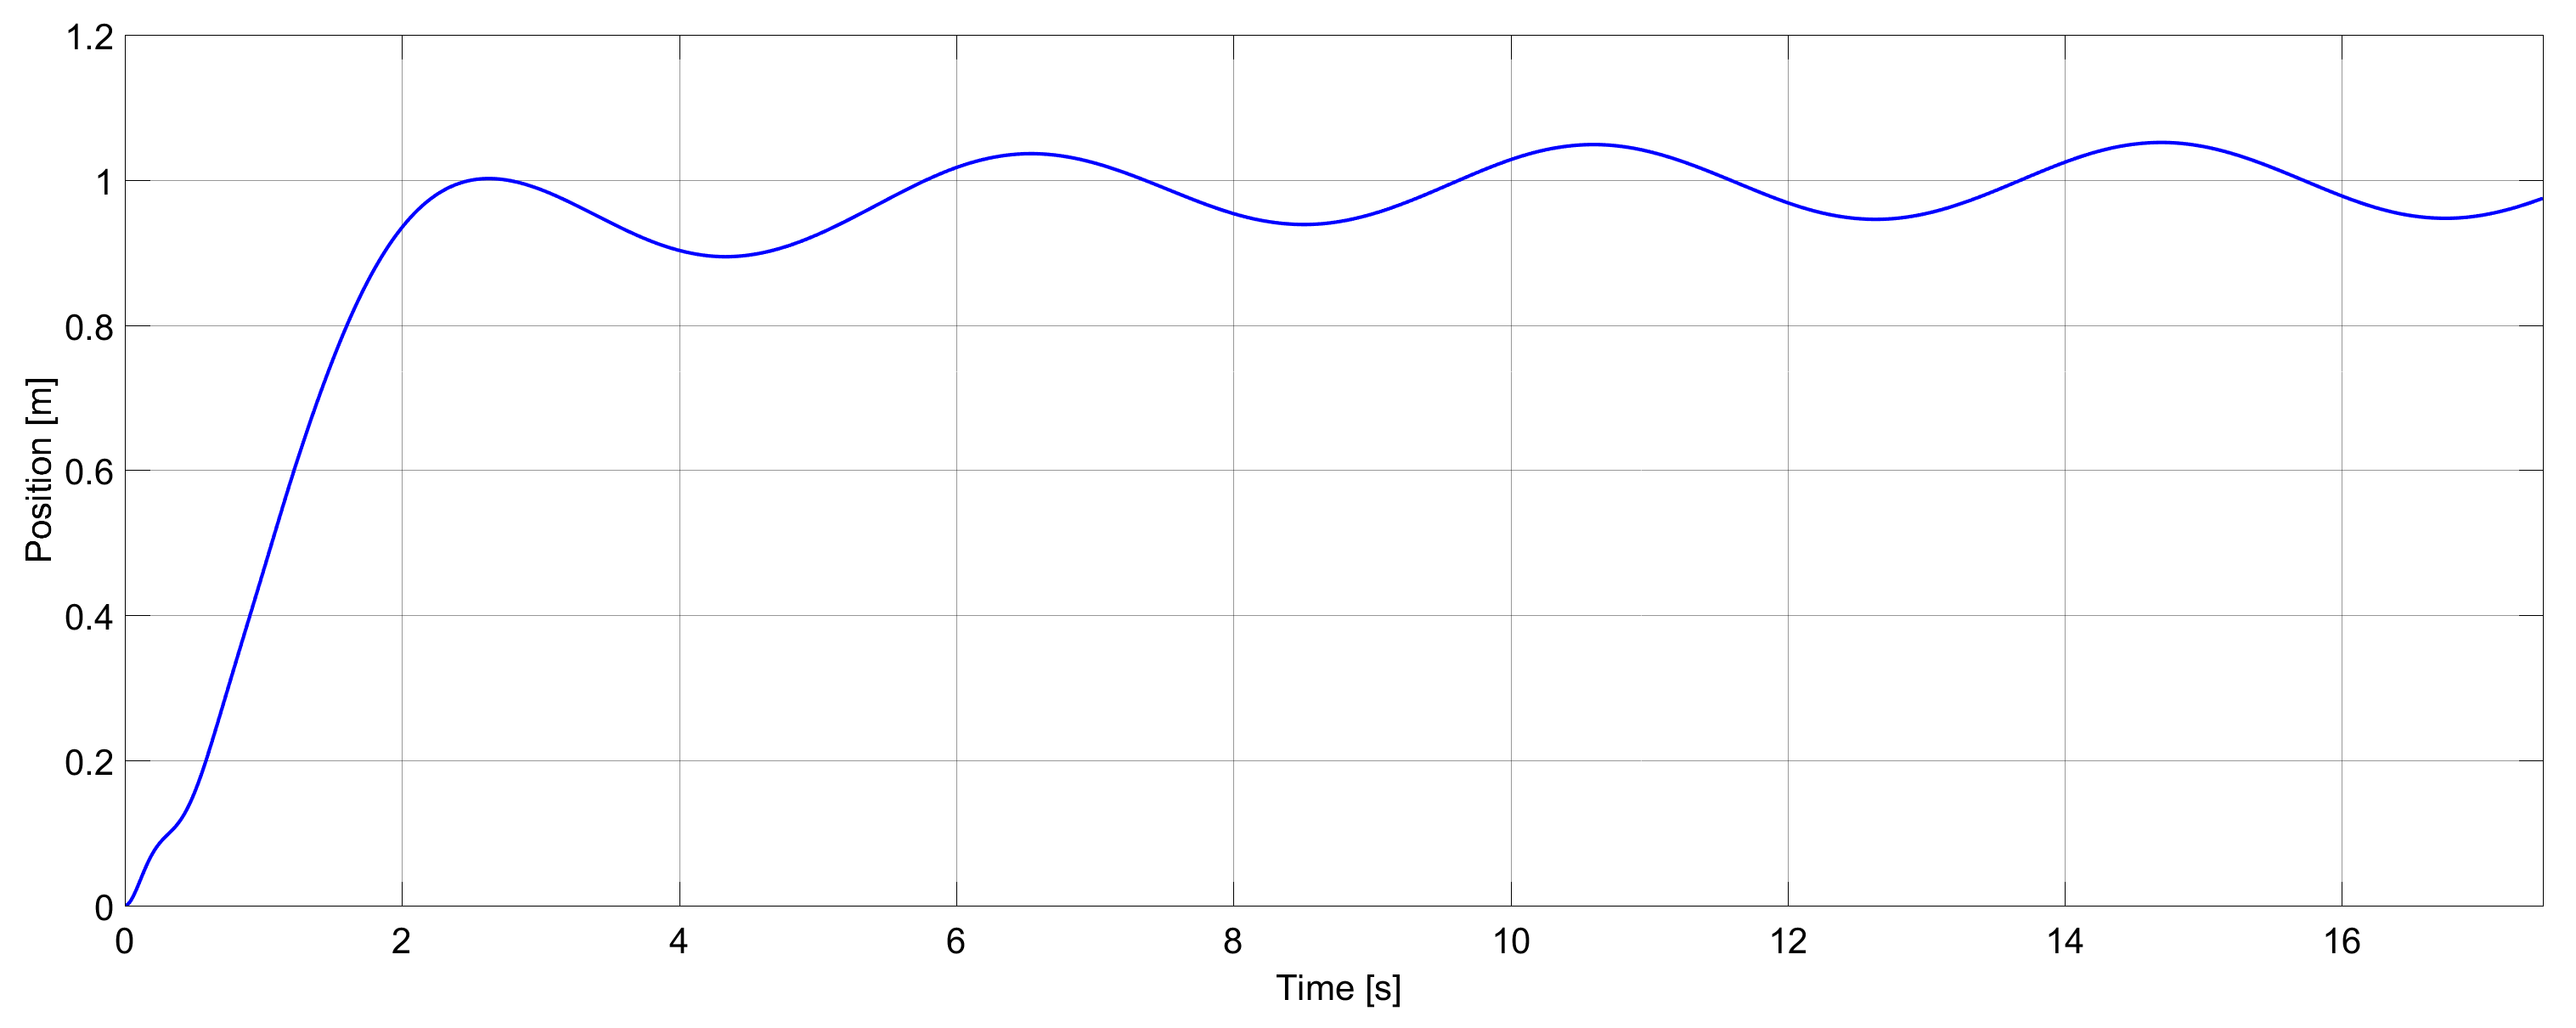
\includegraphics[width=0.8\textwidth]{Billeder/Thomas/100mA}
\end{figure}
\end{frame}


%\subsection{Trolley og pendul model}
% \begin{frame}{Regulator}{Block diagram}


%\begin{columns}[T]
% \begin{column}{.35\textwidth}

%   \begin{itemize}
%     \item<1-> Trolley
%     \vspace{0.8cm}
%     \item<2-> Electromagnetic head 
%     \vspace{1.5cm}
%     \item<3-> Angle sensor
%   \end{itemize}
% \end{column}%
% \hfill%
%\begin{column}{.65\textwidth}

%\vspace{-0.9cm}
%\begin{figure}[H]
%  \centering
% \onslide<1->  \begin{subfigure}{0.98\textwidth}
%         \centering
%         \includegraphics[width=0.5\textwidth]{Billeder/Papilio_DUO}
%         \end{subfigure}

% \onslide<2-> \scalebox{0.8}{ \begin{subfigure}{0.98\textwidth}
%         \centering
%         \begin{figure}[H]

%         \onslide<2-> \scalebox{0.7}{\input{Billeder/Thomas/regulatorblock3.ralf}}
%         \end{figure

%         }

%       \vspace{0.2cm}

%         \begin{figure}[H]

%         \onslide<3-> \scalebox{0.7}{\input{Billeder/Thomas/regulatorblock3.ralf}}
%         \end{figure

%         }




% \onslide<3->  \begin{subfigure}{0.98\textwidth}
%         \centering
%         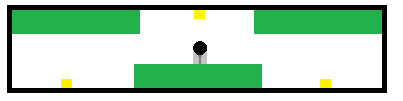
\includegraphics[width=0.5\textwidth]{Billeder/AngleSensor}
%         \end{subfigure}     
% \end{figure}

%\end{column}
%\end{columns}

%\end{frame}

%       \item<1->[] {
%               \begin{figure}[H]
%               \centering
%               \scalebox{0.65}{\input{Billeder/Thomas/regulatorblock3.ralf}}
%               \end{figure}
%       }
%     \end{itemize}           
%   \end{minipage}
%   \\

% %  \input{Billeder/Thomas/regulatorblock3.ralf}
  
% %  \input{Billeder/Thomas/regulatorblock4.ralf}
	  
%   \centering
%   \begin{minipage}[t]{0.75\linewidth}
%     \begin{itemize}
%       \item<1->[] {
%               \begin{figure}[H]
%               \centering
%               \scalebox{0.65}{\input{Billeder/Thomas/regulatorblock4.ralf}}
%               \end{figure}
%       }
%     \end{itemize}           
%   \end{minipage}
%   \\
  
% 	\centering   
%   \begin{minipage}[t]{0.55\linewidth}
    
%     \begin{itemize}
%       \item<1->[] {
%               \begin{figure}[H]
%               \centering
%               \scalebox{0.65}{\input{Billeder/Thomas/regulatorblocky.ralf}}
%               \end{figure}
%       }
%     \end{itemize}           
%   \end{minipage}
  
  
%\end{frame} 